\section{Hadoop}\label{capitolo7}
Al giorno d'oggi produciamo dati ad una velocità impressionante, gli archivi di internet crescono di 20TB al mese, 100TB di dati sono caricati su Facebook ogni giorno. Insieme ai dati di internet crescono anche quelli personali e quelli prodotti dalle macchine.\\
Volendo analizzare questi dati tuttavia si incorrono in diversi problemi, il principale è che le capacità e le velocità dei dischi non sono migliorate di molto negli ultimi anni, tuttavia una soluzione è quella di parallelizzare gli \emph{storage} ma questo comporta problemi di aggregazione dei dati e di replicazione hardware.
Una soluzione a questi problemi potrebbe essere \emph{Hadoop} un sistema di distribuzione dei file che implementa anche un analisi dei dati tramite \emph{map reduce}. A differenza di database relazionali Hadoop non lavora soffre delle latenze dei dischi e non necessita di dati strutturati per lavorare con efficienza, inoltre, il MapReduce scala in maniera lineare. Rispetto al \emph{Volunteer computing} che lavora tramite rete Internet con computer dei quali non si può verificarne l'affidabilità, Hadoop lavora in un cluster locale sfruttando reti ad alte performance.\\
\subsection{La storia}
Nel 2002 Mike Cafarella e Doug Cutting iniziano a lavorare su \emph{Apache Nutch} un nuovo motore di ricerca. Nel 2003 Google pubblica un articolo sul \emph{Google File System} un filesystem distribuito e Mike e Doug iniziano a lavorare ad un progetto simile ma open source. Nel 2004 Google pubblica un ulteriore articolo sul modello di computazione denominato \emph{MapReduce} e ancora una volta Mike e Doug ne implementano una versione open source in Nutch. Nel 2006 questi due progetti si separano da Nutch e diventano \emph{Hadoop}, nello stesso anno Dug inizia a lavorare per "Yahoo!" dove inizia ad usare Handoop. Nel 2008 Yahoo!, Last.fm, Facebook e NYT utilizzano Hadoop. Nel 2009 Yahoo! fa segnare un nuovo record mondiale ordinando 1TB di dati in 62 secondi. Da quel giorno Hadoop è diventato uno standard per l'industria.\\
\subsection{MapReduce}
Il \emph{MapReduce} è un medello per l'analisi di una grande quantità di dati, questi dati sono organizzati come un insieme \emph{chiave-valore}; questo modello si suddivide in due fasi
\begin{itemize}
	\item $map(k_1,v_1) \rightarrow list(k_2,v_2)$  nella quale il dominio di input è diverso dal dominio dell'output
	\item una fase intermedia serve a ordinare la mappa risultante e raggrupparla per chiavi
	\item $reduce(k_2,list(v_2))\rightarrow list(v_3)$ dove il dominio di input e di output coincidono
\end{itemize}
Prima di spiegare in dettaglio il funzionamento doppiamo introdurre alcune definizioni:
\begin{description}
	\item[Job:] è un unità di lavoro eseguita dal sistema che comprende
	\begin{itemize}
		\item dati di input
		\item implementazione del \emph{map} e del \emph{reduce}
		\item configurazione
	\end{itemize}
	\item[Map task e Reduce task:] piccoli frammenti di un job
	\item[Jobtracker:] nodo del cluster che coordina i lavori
	\item[Tasktracker:] esegue un task e restituice il risultato al jobtraker
	\item[Split:] frammento di input
\end{description}
Il jobtracker divide i dati di input in parti e per ogni split di dati viene eseguito un \emph{map task}. Questa esecuzione avviene in parallelo su tutti i nodi, hadoop tenta di eseguire il task di riduzione sulla macchina nel quale risiedono i dati. Il risultato viene scritto sul disco della macchina e non sul HDFS. Il \emph{reduce task} riceve i dati attraverso la rete ed infine il risultato è salvato sull HDFS. In \figurename"\ref{fig:mapreduce} vediamo un esempio di questo procedimento.
\begin{figure}
\centering
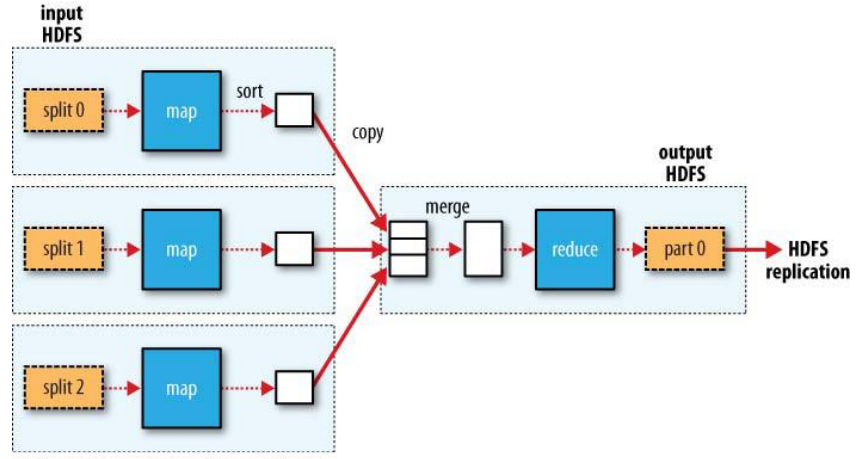
\includegraphics[width=0.7\linewidth]{img/mapreduce}
\caption{Esempio di MapReduce con Hadoop}
\label{fig:mapreduce}
\end{figure}
A volte si rende necessario effettuare delle operazioni sui dati intermedi, le possibile operazioni sono funzioni di combinazione che aggregano i dati per minimizzare il trasferimento sulla rete; e l'operazione di \emph{shuffle} ovvero un ordinamento dei dati di output.\\
In hadoop tutto è configurabile, il numero dei task sia di map che di reduce, la compressione dei dati, la gestione della memoria. Vengono creati dei profili per cercare di capire come migliorare le performance.\\
Per un esempio di come implementare un MapReduce in Hadoop si rimanda a \cite{cugola:hadoop}
\subsection{Hadoop Distributed File System}
\emph{Hadoop Distributed File System} (HDFS) è un filesystem appositamente progettato per lavorare con dati molto grandi ed adatto per accedere ai dati in streaming.
Dalla versione 2 di Hadoop HDFS è composto da un singolo \emph{namenode} (master) e una serie di \emph{datanode}(slave), il namenode gestisce il namespace del filesistem, esso mantiene l'immagine del namespase e scrive i file di log, esso ha inoltre una lista di tutti i datanode e delle informazioni in essi immagazzinate, tuttavia esso non mantiene alcun file.
I datanode sono macchine nelle quali vengono immagazzinati dei blocchi di file, essi comunicano continuamente con il namenode. Ogni file caricato sul HDFS è diviso in blocchi da 64MB in modo da minimizzare lo \emph{seek} e massimizzare il \emph{transfert rate}. Se un blocco è più piccolo di 64MB esso, a differenza di un normale filesystem, non occupa 64MB. Un file potrebbe essere più grande di un singolo disco in rete.\\
Mappers e Reducer utilizzano dei particolari tipi di dato che sono definiti da Hadoop e sono di tipo \emph{wrapping} ovvero ottimizzati per la serializzazione su rete. Per aggiungere nuovi tipi di dato bisogna implementare le due interfacce \texttt{Writeable} e \texttt{WriteableComparable}.
\subsection{PIG}
Pig è un linguaggio che permette l'interrogazione complessa di dati riccamente strutturati. Uno script è una sequenza di trasformazioni sui dati iniziali che può essere tradotta in un \emph{MapReduce job}, è veloce da sviluppare, può essere scritta in poche righe ed eseguita su terabytes di dati.\\
Pig può essere eseguito in tre modi, tramite script, tramite \emph{interactive shell}, oppure embeddato in Java.
\subsection{Approfondimenti}
Per eventuali approfondimenti e alcuni esempi si rimanda alle slide del corso \cite{cugola:hadoop}. Per l'installazione e i tutorial si rimandano alle pagine ufficiali di Hadoop \cite{hadoop:docs} \cite{hadoop:tutorials}